%=====================================================================
%   CHAPTER 2 - LITERATURE REVIEW
%=====================================================================
%   Structure agreed 2026-10-01. Headings only; every section still owes
%   its text. Each TODO lists the points the section is expected to cover.
%
%   HOW TO CITE (natbib). The two forms are NOT interchangeable.
%
%     \citet{key}   TEXTUAL. The author becomes part of the sentence.
%                   "As \citet{shannon1948} showed, ..."
%                   -> As Shannon (1948) showed, ...
%
%     \citep{key}   PARENTHETICAL. The whole citation sits in brackets at
%                   the end of a clause.
%                   "...is a solved problem \citep{shannon1948}."
%                   -> ...is a solved problem (Shannon, 1948).
%
%   \cite{key} behaves like \citet in author-year mode and like a numeric
%   citation in IEEE mode, so it reads differently depending on the switch
%   at the top of 0_main.tex. Prefer \citet and \citep.
%
%   Several sources at once:      \citep{keyA,keyB,keyC}
%   A page or chapter:            \citep[Ch.~8]{key}
%   Year only, author in prose:   \citeyearpar{key}
%
%   thesis.bib currently holds PLACEHOLDER entries only. Replace them.
%=====================================================================
\chapter{Literature Review}
\label{ch:review}

%=====================================================================
\section{Introduction}
\label{sec:ch2.introduction}
\todo{}
%=====================================================================
% TODO: what this chapter covers, in what order, and why that order.
% TODO: state up front that the review builds towards the gap in 2.7.


%=====================================================================
\section{Passive Bistatic Radar}
\label{sec:ch2.pbr}
\todo{}
%=====================================================================
% What is passive bistatic radar? What makes it different from active/monostatic radar?

%---------------------------------------------------------------------
\subsection{Principle of Operation}
\label{subsec:ch2.pbr.principle}
\todo{}
%---------------------------------------------------------------------
% TODO: illuminator of opportunity, non-cooperative transmitter, receiver-only
%       system. Advantages (covert, low cost, no spectrum licence) and
%       disadvantages (no control over the waveform, poor dynamic range).

%---------------------------------------------------------------------
% \subsection{Historical Development of Passive Radar}
% \label{subsec:ch2.pbr.history}
% \todo{}
%---------------------------------------------------------------------
% TODO: Klein Heidelberg, Silent Sentry, Manastash Ridge, the UCT lineage.
% TODO: keep to passive radar; general radar history lives in Chapter 1.

%---------------------------------------------------------------------
\subsection{Bistatic Geometry}
\label{subsec:ch2.pbr.geometry}
\todo{}
%---------------------------------------------------------------------
% TODO: figure of the transmitter-target-receiver triangle (figs/ch2/).
The geometry of a basic, passive bistatic radar is depicted in \ref{fig:bistatic_geometry}. 
\begin{figure}[H]
    \centering
    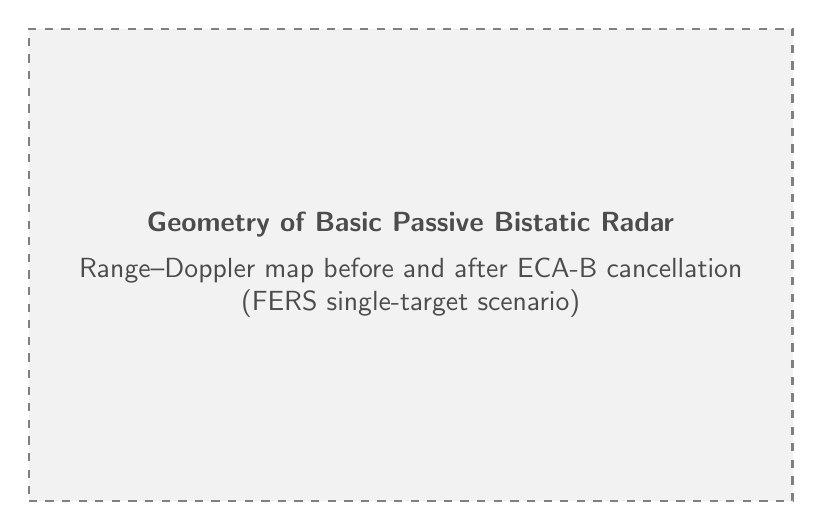
\begin{tikzpicture}
        \node[draw=gray, thick, dashed, fill=gray!10, text=gray!60!black,
              minimum width=0.8\textwidth, minimum height=6cm,
              align=center, font=\sffamily]
        {\textbf{Geometry of Basic Passive Bistatic Radar}\\[1ex]
         Range--Doppler map before and after ECA-B cancellation\\
         (FERS single-target scenario)};
    \end{tikzpicture}
    \caption{\todo{Caption.}}
    \label{fig:bistatic_geometry}
\end{figure}

The radar setup includes a transmitter or illuminator of opportunity, and two receive channels: a referenvce and surveillance.
The reference channel is aimed directly at the illuminator of opportunity such that the direct signal is the strongest one received.
The surveillance antenna is aimed towards some area in which an observed target may be: for example, Cape Town international airport.
The signal received by the surveillance channel is a mixture of the direct (reference) signal, and many other delayed and doppler shifted versions of that direct signal.
Each delayed and doppler shifted "echo" comes from static and dynamic clutter, as well as the moving target itself.
The nature of the receibed signal is one of the mopst important things to understand, because the heaviest part of a passive radar processing chain is designed around filtering out everything except the echoes of the signal reflected off our targets.
In this case, our target is a fast moving aircraft; thus, it's echo will have some magnitude of doppler shift proportional to its velocity.
Other clutter in our scenario also causes echos: static mountains and city infrastructure cause delayed signals arrive. 
Moving trees or ocean waves and clouds may cause delayed and doppler shifted echoes to arrive.

A diagram depicting these various signals is depicted in \ref{fig:signal_echoes}.
\begin{figure}[H]
    \centering
    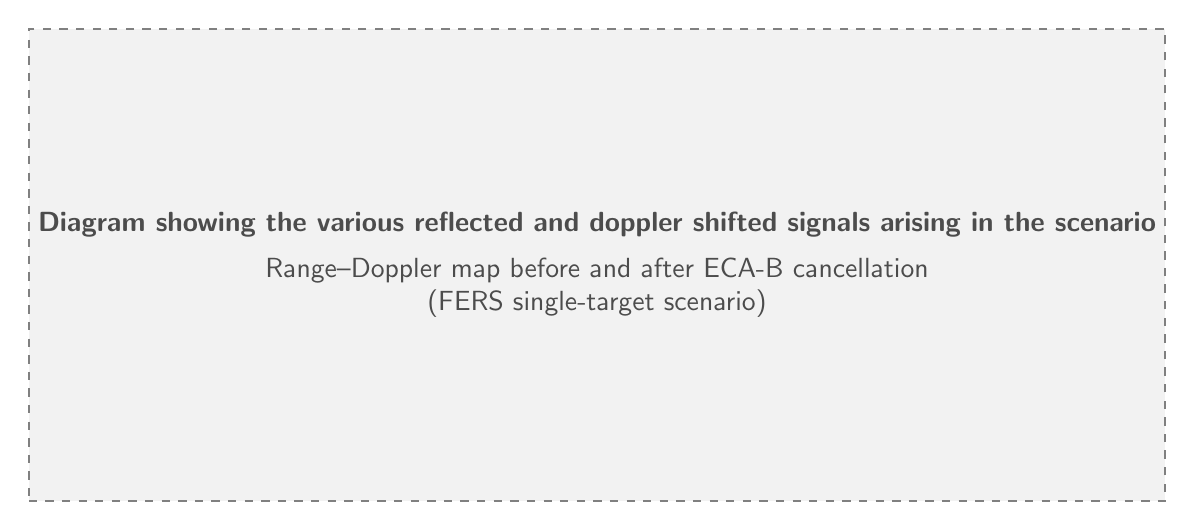
\begin{tikzpicture}
        \node[draw=gray, thick, dashed, fill=gray!10, text=gray!60!black,
              minimum width=0.8\textwidth, minimum height=6cm,
              align=center, font=\sffamily]
        {\textbf{Diagram showing the various reflected and doppler shifted signals arising in the scenario}\\[1ex]
         Range--Doppler map before and after ECA-B cancellation\\
         (FERS single-target scenario)};
    \end{tikzpicture}
    \caption{\todo{Caption.}}
    \label{fig:signal_echoes}
\end{figure}

\subsubsection{Bistatic Range and the Baseline}
\label{subsubsec:ch2.pbr.geometry.range}
\todo{}
% TODO: bistatic range definition, ellipses of constant range, the baseline
%       as the zero-range reference.
Bistatic range is the distance from the transmitter to the target to the receiver...

\subsubsection{Bistatic Doppler}
\label{subsubsec:ch2.pbr.geometry.doppler}
\todo{}
% TODO: bistatic Doppler expression, dependence on the bistatic angle,
%       zero-Doppler cases.

%---------------------------------------------------------------------
\subsection{Signal Model}
\label{subsec:ch2.pbr.signalmodel}
\todo{}
%---------------------------------------------------------------------

\subsubsection{Reference and Surveillance Channels}
\label{subsubsec:ch2.pbr.signalmodel.channels}
\todo{}
% TODO: two-channel receiver, purpose of each channel, reference purity.

\subsubsection{Direct Signal, Multipath and Clutter}
\label{subsubsec:ch2.pbr.signalmodel.clutter}
\todo{}
% TODO: composition of the surveillance channel; stationary clutter as
%       delayed copies of the reference at zero Doppler.

\subsubsection{Target Echoes}
\label{subsubsec:ch2.pbr.signalmodel.targets}
\todo{}
% TODO: delayed and Doppler-shifted copies; relative power to the direct
%       signal; where the bistatic radar equation enters.
\begin{equation}
    P_r = \frac{P_t \, G_t \, G_r \, \lambda^2 \, \sigma_b \, F_t^2 \, F_r^2}
               {(4\pi)^3 \, R_T^2 \, R_R^2 \, L_t \, L_r}
    \label{eq:bistatic-radar}
\end{equation}

\begin{figure}[H]
    \centering
    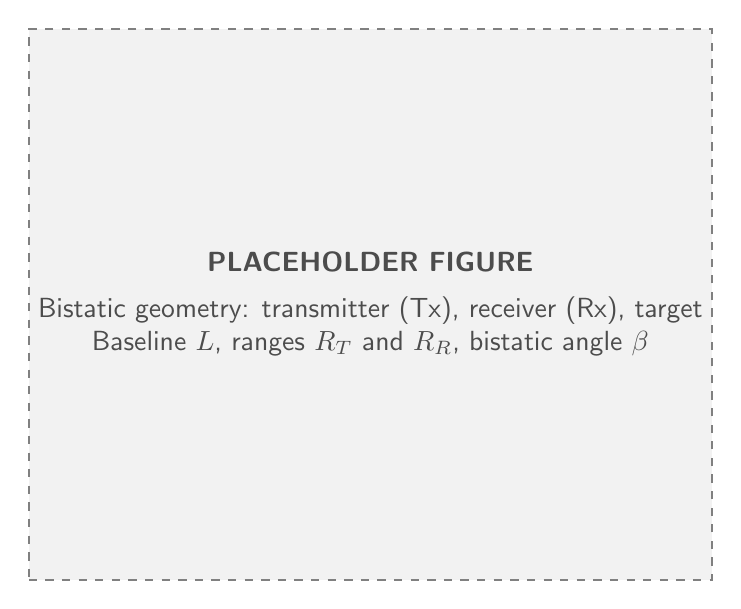
\begin{tikzpicture}
        \node[draw=gray, thick, dashed, fill=gray!10, text=gray!60!black,
              minimum width=0.7\textwidth, minimum height=7cm,
              align=center, font=\sffamily]
        {\textbf{PLACEHOLDER FIGURE}\\[1ex]
         Bistatic geometry: transmitter (Tx), receiver (Rx), target\\
         Baseline $L$, ranges $R_T$ and $R_R$, bistatic angle $\beta$};
    \end{tikzpicture}
    \caption{\todo{Caption.}}
    \label{fig:bistatic-geometry}
\end{figure}

%---------------------------------------------------------------------
\subsection{FM Broadcast as an Illuminator of Opportunity}
\label{subsec:ch2.pbr.fm}
\todo{}
%---------------------------------------------------------------------
% SEE Report/docs/fm_broadcast_summary.md
\subsubsection{Properties of the FM Waveform}
\label{subsubsec:ch2.pbr.fm.waveform}
\todo{}
% TODO: band, channel spacing, transmitter power and coverage, continuous
%       transmission, why FM suits long-range air surveillance.

\subsubsection{Ambiguity Function and Content Dependence}
\label{subsubsec:ch2.pbr.fm.ambiguity}
\todo{}
% TODO: instantaneous bandwidth varies with programme content; effect on
%       sidelobes; speech vs music; the ambiguity-function literature.

\subsubsection{Range and Doppler Resolution}
\label{subsubsec:ch2.pbr.fm.resolution}
\todo{}
% TODO: resolution from bandwidth and integration time; typical figures,
%       each with a citation.

%---------------------------------------------------------------------
% \subsection{Aircraft as Targets at FM Frequencies}
% \label{subsec:ch2.pbr.aircraft}
% \todo{}
%---------------------------------------------------------------------

\subsubsection{Radar Cross-Section}
\label{subsubsec:ch2.pbr.aircraft.rcs}
\todo{}
% TODO: RCS of commercial aircraft at VHF, resonance-region behaviour.

\subsubsection{Expected Doppler and Range Extents}
\label{subsubsec:ch2.pbr.aircraft.extents}
\todo{}
% TODO: speeds and altitudes of aircraft near an airport; the Doppler and
%       bistatic-range window this sets for the map.

%---------------------------------------------------------------------
\subsection{The Dynamic-Range Problem}
\label{subsec:ch2.pbr.dynamicrange}
\todo{}
%---------------------------------------------------------------------
% TODO: direct-signal to echo power ratio; masking through the ambiguity
%       sidelobes; why cancellation is needed before correlation.
% TODO: this subsection is the hinge into 2.3.2.


%=====================================================================
\section{The Passive Radar Processing Chain}
\label{sec:ch2.chain}
\todo{}
%=====================================================================
This section details the processing algorithms involved in passive radar processing. Taking the received reference and surveillance channel signals, and ending up with an amplitude-range-doppler map that should reveal a moving target.

%---------------------------------------------------------------------
\subsection{Overview of the Chain}
\label{subsec:ch2.chain.overview}
\todo{}
%---------------------------------------------------------------------
% TODO: block diagram (figs/ch2/): receive, condition, cancel, correlate,
%       detect, track/display. Name which blocks this thesis implements.
A block diagram of the passive radar processing chain used in this project is shown below in \ref{fig:processing-chain-diagram}.

\begin{figure}[H]
    \centering
    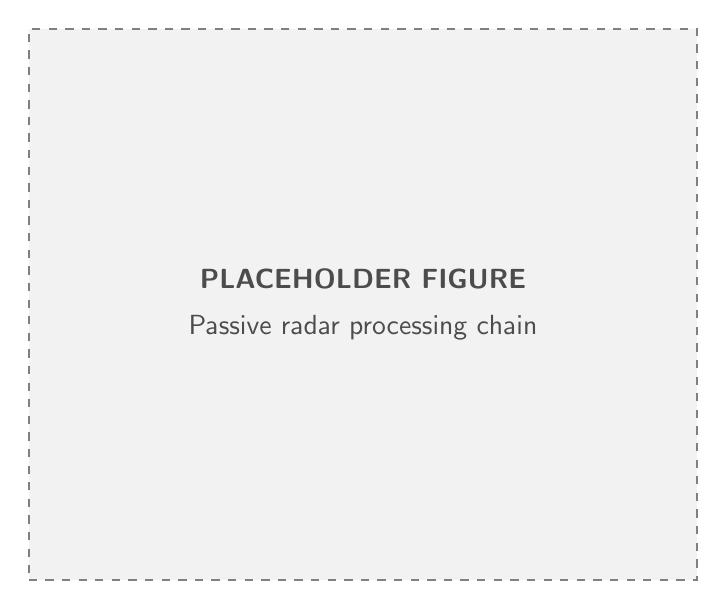
\begin{tikzpicture}
        \node[draw=gray, thick, dashed, fill=gray!10, text=gray!60!black,
              minimum width=0.7\textwidth, minimum height=7cm,
              align=center, font=\sffamily]
        {\textbf{PLACEHOLDER FIGURE}\\[1ex]
         Passive radar processing chain};
    \end{tikzpicture}
    \caption{\todo{Caption.}}
    \label{fig:processing-chain-diagram}
\end{figure}

Describe ...
%---------------------------------------------------------------------
\subsection{Direct-Signal Interference Cancellation}
\label{subsec:ch2.chain.dsi}
\todo{}
%---------------------------------------------------------------------
The first and most important part of passive radar processing is filtering out the direct FM signal received by the reference channel which is many order of magnitude stronger than the target echo which we are looking for.
Not only does the surveillance antenna still hear the direct signal, it also receives the transmitted signal reflections of buildings, hills and infrastructure -- each with a unique time delay.
The direct signal and building reflections are roughly a million times stronger than the target (aircraft echo).
The DSI processing stage aims to remove the direct signal and clutter so that the echo from the aircraft target is clearer.

\subsubsection{Formulation as a Least-Squares Problem}
\label{subsubsec:ch2.chain.dsi.leastsquares}
\todo{}
% TODO: clutter subspace spanned by delayed reference copies; the normal
%       equations; the projection interpretation shared by the ECA family.
The target echo can be found by subtracting the received surveillance signal by the emount of "clutter" that it contains. And such "clutter" can be modeled as the sum of delayed and doppler shifted copes of the reference signal.
As such, we get the equation
$ target[n] = s[n] - (w[0] \cdot r[n] + w[1] \cdot r[n-1] + w[2] \cdot r[n-2] + ... + w[N] \cdot r[n-N] )$
Where ... state what each variable means.
% This equation needs to be labelled.
We want the scale factors $w$ that leave the most energy behind; thus, this is a least-squares problem with a closed form answer:
The Gram matrix, $G$ has entries $G[i][j]$ that represent how similar the reference delayed by $i$ is to the reference delayed by $j$.
The right-hand side, $v$ has entries $v[i]$ that represent how similar the reference delayed by i is to the surveillance signal. This is effectively a map of how the clutter is dispersed in the scenario physically.
The answer to the problem is a solution of euqation ... label:

$G \cdot w = v$

Each variant of a DSI algorithm focuses on solving for this solution: an $N \times N$ system of equations.

\subsubsection{Extensive Cancellation Algorithm (ECA)}
\label{subsubsec:ch2.chain.dsi.eca}
\todo{}
% TODO: original formulation; cost of the full-CPI solve.

\subsubsection{Batched ECA (ECA-B)}
\label{subsubsec:ch2.chain.dsi.ecab}
\todo{}
% TODO: splitting the CPI into batches; effect on cost and on Doppler
%       notch width.

\subsubsection{Sliding ECA (ECA-S)}
\label{subsubsec:ch2.chain.dsi.ecas}
\todo{}
% TODO: overlapping windows; what it buys over ECA-B and what it costs.

\subsubsection{ECA by Carrier and Doppler (ECA-CD)}
\label{subsubsec:ch2.chain.dsi.ecacd}
\todo{}
% TODO: extending the subspace to non-zero Doppler; when that is needed.

\subsubsection{Conjugate Gradient Least Squares (CGLS)}
\label{subsubsec:ch2.chain.dsi.cgls}
\todo{}
% TODO: iterative solution of the same least-squares problem; convergence;
%       semiconvergence in finite precision; iteration count as a knob.

\subsubsection{Adaptive Filtering Approaches}
\label{subsubsec:ch2.chain.dsi.adaptive}
\todo{}
% TODO: LMS, NLMS, FBLMS; convergence vs tracking; why they are reviewed
%       but not benchmarked here (or why they are, if that changes).

\subsubsection{Comparison of Methods}
\label{subsubsec:ch2.chain.dsi.comparison}
\todo{}
% TODO: table comparing cost, suppression and latency as reported in the
%       literature. State which methods are carried forward and why.

%---------------------------------------------------------------------
\subsection{Range-Doppler Map Formation}
\label{subsec:ch2.chain.ard}
\todo{}
%---------------------------------------------------------------------

\subsubsection{The Cross-Ambiguity Function}
\label{subsubsec:ch2.chain.ard.caf}
\todo{}
% TODO: definition; the map as a matched filter bank over delay and Doppler.

\subsubsection{Time-Domain Correlation}
\label{subsubsec:ch2.chain.ard.timedomain}
\todo{}
% TODO: direct evaluation; cost.

\subsubsection{Frequency-Domain Correlation}
\label{subsubsec:ch2.chain.ard.freqdomain}
\todo{}
% TODO: FFT-based correlation; cost.

\subsubsection{Batched Correlation}
\label{subsubsec:ch2.chain.ard.batched}
\todo{}
% TODO: batch-and-FFT method; approximation made; Doppler resolution limits.

\subsubsection{Computational Complexity}
\label{subsubsec:ch2.chain.ard.complexity}
\todo{}
% TODO: side-by-side operation counts; this justifies the choice in Ch. 3.

%---------------------------------------------------------------------
\subsection{Constant False Alarm Rate Detection}
\label{subsec:ch2.chain.cfar}
\todo{}
%---------------------------------------------------------------------

\subsubsection{Cell-Averaging CFAR}
\label{subsubsec:ch2.chain.cfar.ca}
\todo{}
% TODO: reference window, guard cells, threshold factor, P_fa relation.

\subsubsection{Two-Dimensional CFAR}
\label{subsubsec:ch2.chain.cfar.2d}
\todo{}
% TODO: extension to the range-Doppler map; window shape; edge handling.

\subsubsection{Variants and Their Trade-offs}
\label{subsubsec:ch2.chain.cfar.variants}
\todo{}
% TODO: GO, SO, OS-CFAR; clutter edges and multiple targets; why CA is used.


% %=====================================================================
% \section{Performance Evaluation of Passive Radar}
% \label{sec:ch2.evaluation}
% \todo{}
% %=====================================================================

% %---------------------------------------------------------------------
% \subsection{Measures of Cancellation Performance}
% \label{subsec:ch2.evaluation.cancellation}
% \todo{}
% %---------------------------------------------------------------------
% % TODO: clutter attenuation, residual power, suppression in dB; how each is
% %       defined in the literature and which definition this thesis adopts.

% %---------------------------------------------------------------------
% \subsection{Measures of Detection Performance}
% \label{subsec:ch2.evaluation.detection}
% \todo{}
% %---------------------------------------------------------------------
% % TODO: P_d, P_fa, SNR on the map; detection range.

% %---------------------------------------------------------------------
% \subsection{Processing Latency and Real-Time Constraints}
% \label{subsec:ch2.evaluation.latency}
% \todo{}
% %---------------------------------------------------------------------
% % TODO: what "real time" means for a CPI-based system; how others report
% %       timing; warm-up and clock pinning as reporting caveats.

% %---------------------------------------------------------------------
% \subsection{ADS-B as Ground Truth}
% \label{subsec:ch2.evaluation.adsb}
% \todo{}
% %---------------------------------------------------------------------
% % TODO: what ADS-B provides; prior use for validating passive radar;
% %       limitations (coverage, latency, non-equipped aircraft).

% %---------------------------------------------------------------------
% \subsection{Simulation for Verification}
% \label{subsec:ch2.evaluation.simulation}
% \todo{}
% %---------------------------------------------------------------------
% % TODO: FERS; golden-reference verification against MATLAB.
% % TODO: drop this subsection if Chapter 3 covers it fully.


%=====================================================================
\section{Real-Time and Embedded Implementations}
\label{sec:ch2.implementations}
\todo{}
%=====================================================================

%---------------------------------------------------------------------
\subsection{GPU-Based Passive Radar Processing}
\label{subsec:ch2.implementations.gpu}
\todo{}
%---------------------------------------------------------------------
% TODO: desktop-GPU implementations; which stages were ported; speed-ups
%       reported and against what baseline.

%---------------------------------------------------------------------
\subsection{Embedded and Single-Board Implementations}
\label{subsec:ch2.implementations.embedded}
\todo{}
%---------------------------------------------------------------------
% TODO: Jetson and other SBC passive radar work; memory and power limits.

%---------------------------------------------------------------------
\subsection{The Previous UCT FM Passive Radar System}
\label{subsec:ch2.implementations.uct}
\todo{}
%---------------------------------------------------------------------

\subsubsection{System Architecture}
\label{subsubsec:ch2.implementations.uct.architecture}
\todo{}
% TODO: receiver, PXGF transport, processing server, ARDView; cite Tong.

\subsubsection{The CUDA Processing Server}
\label{subsubsec:ch2.implementations.uct.cudaprocserver}
\todo{}
% TODO: what it did on the TK1; what survives (docs/legacy-audit.md).

\subsubsection{Limitations}
\label{subsubsec:ch2.implementations.uct.limitations}
\todo{}
% TODO: what the old system could not do and what motivates the upgrade.


% %=====================================================================
% \section{Hardware Platforms}
% \label{sec:ch2.hardware}
% \todo{}
% %=====================================================================

% %---------------------------------------------------------------------
% \subsection{Software-Defined Radio Receivers}
% \label{subsec:ch2.hardware.sdr}
% \todo{}
% %---------------------------------------------------------------------

% \subsubsection{The USRP2 and BasicRX Front End}
% \label{subsubsec:ch2.hardware.sdr.usrp2}
% \todo{}
% % TODO: architecture, ADC, DDC, two-channel coherent receive, UHD.

% \subsubsection{VITA 49 Sample Transport}
% \label{subsubsec:ch2.hardware.sdr.vita49}
% \todo{}
% % TODO: the standard, signal data and context packets, timestamps; why it
% %       replaces PXGF.

% %---------------------------------------------------------------------
% \subsection{GPU Computing with CUDA}
% \label{subsec:ch2.hardware.cuda}
% \todo{}
% %---------------------------------------------------------------------

% \subsubsection{Programming Model}
% \label{subsubsec:ch2.hardware.cuda.model}
% \todo{}
% % TODO: kernels, grids and blocks, memory hierarchy, host-device transfers,
% %       unified memory on Tegra.

% \subsubsection{Precision on Embedded GPUs}
% \label{subsubsec:ch2.hardware.cuda.precision}
% \todo{}
% % TODO: FP32 vs FP64 throughput on Maxwell; consequence for CGLS.

% \subsubsection{cuFFT, cuBLAS and cuSOLVER}
% \label{subsubsec:ch2.hardware.cuda.libraries}
% \todo{}
% % TODO: what each provides and which stage uses it.

% %---------------------------------------------------------------------
% \subsection{NVIDIA Jetson TK1}
% \label{subsec:ch2.hardware.tk1}
% \todo{}
% %---------------------------------------------------------------------
% % TODO: Tegra K1 specification from the datasheet; the platform of the old
% %       system.

% %---------------------------------------------------------------------
% \subsection{NVIDIA Jetson Nano}
% \label{subsec:ch2.hardware.nano}
% \todo{}
% %---------------------------------------------------------------------
% % TODO: Tegra X1 specification from the datasheet; L4T, CUDA 10.2 ceiling.

% %---------------------------------------------------------------------
% \subsection{Platform Comparison}
% \label{subsec:ch2.hardware.comparison}
% \todo{}
% %---------------------------------------------------------------------
% % TODO: table TK1 vs Nano (CUDA cores, architecture, FP32 rate, memory,
% %       bandwidth, power). Every figure cited to a datasheet in the caption.
% % \begin{table}[H]
% %     \centering
% %     \caption[Platform comparison]{\textbf{Platform comparison.} TODO}
% %     \label{table:ch2.platformcomparison}
% % \end{table}


%=====================================================================
\section{Summary and Research Gap}
\label{sec:ch2.summary}
\todo{}
%=====================================================================
% TODO: what the literature establishes; what it does not answer (DSI
%       cancellers compared on one embedded GPU, suppression vs latency);
%       tie each gap to an objective in Chapter 1.

%****************************************************
% END
%****************************************************
